\section{PCB under test}
\label{sec:pcb-overview}
The measurements described in this chapter characterise the cross-talk and capacitance of a PCB designed for the ALLEGRO barrel calorimeter (Figure~\ref{fig:pcb}). This note is based on cern PCB v2 and China PCB v1. For measurements of an endcap PCB or a different board layout, update the topology-dependent channel maps and geometry parameters in the analysis scripts before using them.

\subsection{Tower layouts}
The board contains 16 towers with different signal-routing layouts or structural features. Towers 1, 2, 15 and 16 explore different strip-layer sizes or positions; the other towers explore different signal-path matching and shielding arrangements. Refer to the PCB layout drawing for the detailed configuration of each tower.

Each tower has a 16-pin connector. With the connector at the top of the board, the connector channels are numbered from right to left, from 1 to 16. In the logical-trace (\code{logTrac}) layout, cell 1 is the cell farthest from the connector. The channel-to-cell mapping follows the cell order, starting with channel 1 for cell 1, with channel 8 skipped. For the optimal-trace layout, use the tower-specific mappings in \code{default_config.m}; the maps currently implemented in the toolkit are listed in Section~\ref{sec:tower-maps}.

Connector-channel numbering must be distinguished from the toolkit's acquisition-channel and display conventions described in Section~\ref{sec:channel-conventions}.
\todo{Add an annotated connector pinout showing how all 16 connector channels correspond to the 15 acquisition channels, including the role of channel 8 and the exact cell numbering after it is skipped. Identify the viewed side of the PCB so that right-to-left numbering is unambiguous.}

\subsection{Scope of the measurements}
The toolkit supports two measurements: a cross-talk matrix and a per-channel capacitance measurement. Each tower has 15 acquisition channels. A full cross-talk scan records all 225 injection/readout combinations. A capacitance scan records 15 waveforms with injection and readout routed to the same channel. Capacitance is obtained offline by comparing the fitted time constants with a separately acquired T0 reference.

The multiplexer selects channels within the connected tower. It does not change the physical tower connection. The operator must reconnect the apparatus and update the tower number between towers.
\todo{Record the board revision and add the PCB layout drawing with tower identifiers. Explain the construction and electrical meaning of the T0 reference.}

\begin{figure}[p]
    \centering
    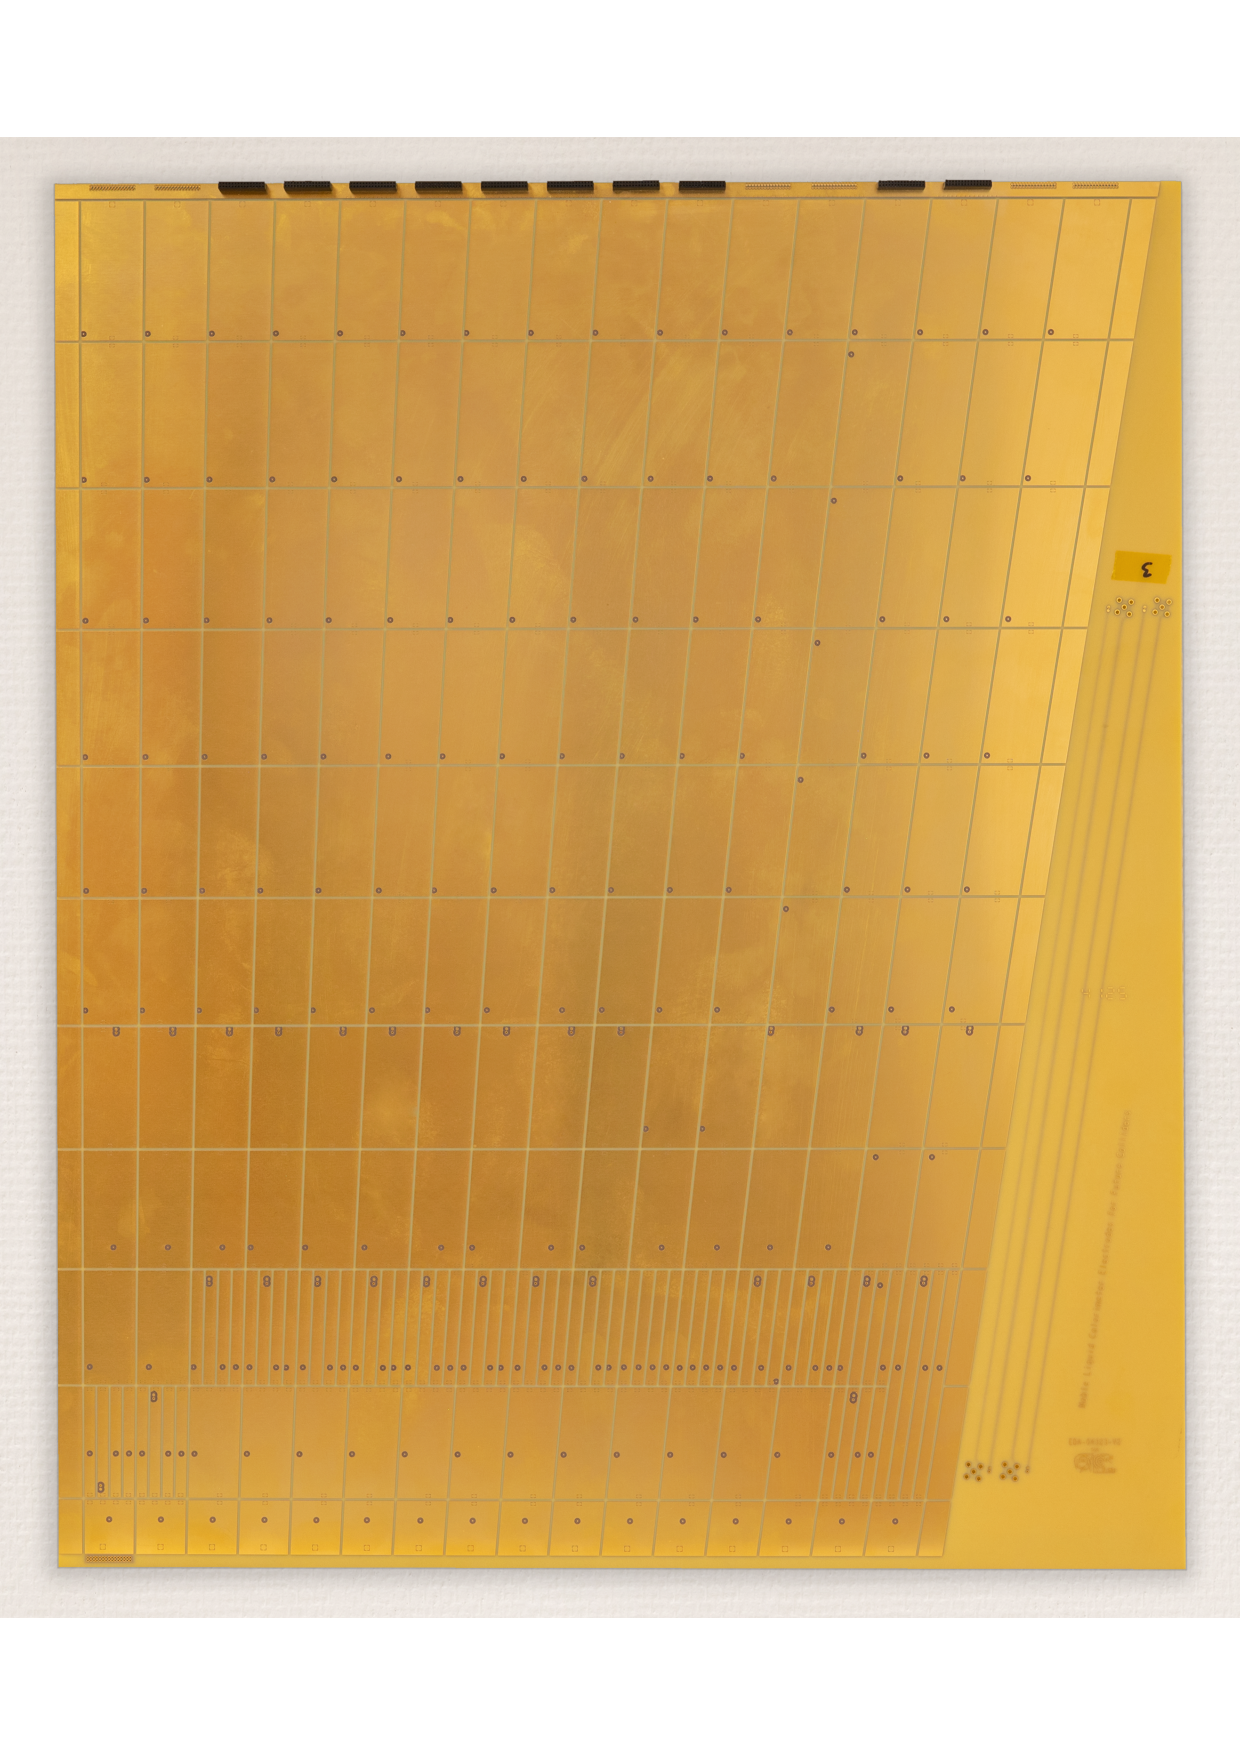
\includegraphics[width=\linewidth,height=0.82\textheight,keepaspectratio]{figures/PCB_ver2.pdf}
    \caption{ALLEGRO barrel calorimeter PCB with 16 towers. The connectors are along the upper edge in this view. Refer to the PCB layout drawing for tower identifiers and routing details.}
    \label{fig:pcb}
\end{figure}

\section{Measurement setup and conventions}
\label{sec:setup}
\subsection{Signal path and instrument roles}
The acquisition software assumes that oscilloscope CH1 carries the direct generator reference and CH2 carries the multiplexer readout. The scripts configure and read CH2 only. CH1 and the trigger are set on the instrument by the operator. The exact generator branching, loading and connector arrangement must be documented from the bench.
\placeholder{Insert an annotated wiring diagram and a photograph of the connected setup.}{Setup documentation to be added. Label generator output, reference branch, injection path, readout path, multiplexer connectors, tower orientation and scope inputs.}

\begin{tabularx}{\linewidth}{@{}lX@{}}
\toprule
Element & Role and information to record \\
\midrule
Signal generator & Excitation source; model, output mode, amplitude convention and load. \\
Multiplexer & Routes injection and readout channels; model, connector pinout and GPIB address. \\
Oscilloscope & Single-shot capture of CH2; model, firmware, input settings and trigger. \\
Windows PC & VISA communication and MATLAB acquisition. \\
Offline computer & MATLAB analysis and result export; may be separate from the acquisition PC. \\
\bottomrule
\end{tabularx}
\todo{Add instrument models and serial numbers, generator waveform/frequency/amplitude/offset, termination and probe settings, scope coupling and bandwidth, sample rate, record length, time window and trigger settings. Cross-talk and capacitance may need separate setup records.}

\subsection{Three channel-number conventions}
\label{sec:channel-conventions}
An \emph{acquisition channel} is the number 1--15 passed to the multiplexer. A \emph{display position} follows \code{cfg.displayOrder}; position 8 is omitted from the cross-talk heatmap after reordering. A \emph{study cell} follows the separate \code{cfg.studyCellToChannel} map. These conventions must be kept distinct when comparing a plotted cell with a physical connector.

The cross-talk scan's adjacent-pair preset is selected by
\[
 |i-j|=1,
\]
where $i$ and $j$ are acquisition-channel numbers. This condition alone does not establish physical adjacency on the PCB.
\todo{Complete the connector-to-acquisition-channel map introduced in Section~\ref{sec:pcb-overview}, explain why display position 8 is omitted, and identify physical neighbours for each board layout.}
